% Template file for an a0 landscape poster.
% Written by Graeme, 2001-03 based on Norman's original microlensing
% poster.
%
% See discussion and documentation at
% <http://www.astro.gla.ac.uk/users/norman/docs/posters/> 
%
% $Id: poster-template-landscape.tex,v 1.2 2002/12/03 11:25:46 norman Exp $


% Default mode is landscape, which is what we want, however dvips and
% a0poster do not quite do the right thing, so we end up with text in
% landscape style (wide and short) down a portrait page (narrow and
% long). Printing this onto the a0 printer chops the right hand edge.
% However, 'psnup' can save the day, reorienting the text so that the
% poster prints lengthways down an a0 portrait bounding box.
%
% 'psnup -w85cm -h119cm -f poster_from_dvips.ps poster_in_landscape.ps'

\documentclass[a0]{a0poster}
% You might find the 'draft' option to a0 poster useful if you have
% lots of graphics, because they can take some time to process and
% display. (\documentclass[a0,draft]{a0poster})
\input{defs.tex}
\pagestyle{empty}
\setcounter{secnumdepth}{0}
\renewcommand{\familydefault}{\sfdefault}
\newcommand{\QED}{~~\rule[-1pt]{8pt}{8pt}}\def\qed{\QED}

\renewcommand{\reals}{{\mbox{\bf R}}}

% The textpos package is necessary to position textblocks at arbitary 
% places on the page.
\usepackage[absolute]{textpos}

\usepackage{amsmath}
\usepackage{hyperref}

\usepackage{fleqn,psfrag,wrapfig,tikz}

\usepackage[papersize={38in,28in}]{geometry}

% Graphics to include graphics. Times is nice on posters, but you
% might want to switch it off and go for CMR fonts.
\usepackage{graphics}


% we are running pdflatex, so convert .eps files to .pdf
%\usepackage[pdftex]{graphicx}
%\usepackage{epstopdf}

% These colours are tried and tested for titles and headers. Don't
% over use color!
\usepackage{color}
\definecolor{Red}{rgb}{0.9,0.0,0.1}

\definecolor{bluegray}{rgb}{0.15,0.20,0.40}
\definecolor{bluegraylight}{rgb}{0.35,0.40,0.60}
\definecolor{gray}{rgb}{0.3,0.3,0.3}
\definecolor{lightgray}{rgb}{0.7,0.7,0.7}
\definecolor{darkblue}{rgb}{0.2,0.2,1.0}
\definecolor{darkgreen}{rgb}{0.0,0.5,0.3}

\renewcommand{\labelitemi}{\textcolor{bluegray}\textbullet}
\renewcommand{\labelitemii}{\textcolor{bluegray}{--}}

\setlength{\labelsep}{0.5em}


% see documentation for a0poster class for the size options here
\let\Textsize\normalsize
%\def\Head#1{\noindent\hbox to \hsize{\hfil{\LARGE\color{bluegray} #1}}\bigskip}
\def\Head#1{\noindent{\LARGE\color{bluegray} #1}\bigskip}
\def\LHead#1{\noindent{\LARGE\color{bluegray} #1}\bigskip}
\def\Subhead#1{\noindent{\large\color{bluegray} #1}\bigskip}
\def\Title#1{\noindent{\VeryHuge\color{Red} #1}}


% Set up the grid
%
% Note that [40mm,40mm] is the margin round the edge of the page --
% it is _not_ the grid size. That is always defined as 
% PAGE_WIDTH/HGRID and PAGE_HEIGHT/VGRID. In this case we use
% 23 x 12. This gives us three columns of width 7 boxes, with a gap of
% width 1 in between them. 12 vertical boxes is a good number to work
% with.
%
% Note however that texblocks can be positioned fractionally as well,
% so really any convenient grid size can be used.
%
\TPGrid[40mm,40mm]{23}{12}      % 3 cols of width 7, plus 2 gaps width 1

\parindent=0pt
\parskip=0.2\baselineskip

\begin{document}

% Understanding textblocks is the key to being able to do a poster in
% LaTeX. In
%
%    \begin{textblock}{wid}(x,y)
%    ...
%    \end{textblock}
%
% the first argument gives the block width in units of the grid
% cells specified above in \TPGrid; the second gives the (x,y)
% position on the grid, with the y axis pointing down.

% You will have to do a lot of previewing to get everything in the 
% right place.

% This gives good title positioning for a portrait poster.
% Watch out for hyphenation in titles - LaTeX will do it
% but it looks awful.
\begin{textblock}{23}(-0.01,0)
\Title{Neural methods for solving calculus of variation problems}
\end{textblock}

\begin{textblock}{23}(0,0.6)
{
\LARGE
Yury Prokhorov
}

{
\Large
\color{bluegray}
\emph{Optimization Class Project. MIPT}
}
\end{textblock}


% Uni logo in the top right corner. A&A in the bottom left. Gives a
% good visual balance, but you may want to change this depending upon
% the graphics that are in your poster.
%\begin{textblock}{2}(0,10)
%Your logo here
%%\includegraphics{/usr/local/share/images/AandA.epsf}
%\end{textblock}

%\begin{textblock}{2}(21.2,0)
%Another logo here
%%\resizebox{2\TPHorizModule}{!}{\includegraphics{/usr/local/share/images/GUVIu/GUVIu.eps}}
%\end{textblock}


\begin{textblock}{6.5}(0,1.5)

\hrule\medskip
\Head{Introduction}\\
A calculus of variations problem is minimizing an integral functional over a given set of functions. Such problems naturally arise in many practical engineering cases. A general way of tackling them involves solving an Euler-Lagrange equation which is a second order differential equation. In many cases the complexity of this equation does not allow for a solution by quadratures, thus, numerical methods are necessary.\\\\[-1em]
Generally, numerical methods are categorized as direct and indirect methods. Direct methods convert a problem into a finite dimensional one, while indirect methods attempt to find a solution of an Euler-Lagrange equation. In present work a direct method using neural networks is proposed.

\medskip\smallskip
\hrule\medskip
\Head{Problem statement}\\
An optimization problem is stated as follows
$$J[x(t)] = \int\limits_{t_0}^{t_\text{f}} L\big(t, x(t), \dot{x}(t)\big) \, dt \longrightarrow \min_{x(t)}$$
where $x(t)$ is a differentiable function on interval $[t_0, t_\text{f}]$.\\\\
Often boundary conditions are added:
$$x(t_0) = x_0, \qquad x(t_\text{f}) = x_\text{f}$$
There also are other variations in which one or both boundary conditions are missing, or there is an extra integral condition (isoperimetric problem).

\medskip
\hrule\medskip
\Head{Discretization}\\
There are two continuous features that are evaluated numerically:
\begin{enumerate}
\item Derivative $\dot{x}(t)$.\\\\[-1em]
It can be estimated using finite differences. In present work the central differences method is used: $\dot{x}(t) \approx \frac{x(t+h) - x(t-h)}{2h}$.
\item Integral $J[x]$.\\\\[-1em]
The integral can be evaluated using numerical methods with an $N$ points split. In present work trapezoid rule and Simpson's rule are applied.
\end{enumerate}
The problem is reduced to minimizing $\widehat{J}(x)$, where $\widehat{J}$ is a numerical approximation of the integral and $x$ is a finite dimensional vector whose components are used to compute $\widehat{J}$ and $\dot{x}$.\\\\
The dimensionality of such problem is $\mathcal{O}(N)$. However, knowing that components of $x$ should form a smooth function, we can reduce the problem to $\mathcal{O}(1)$ by approximating a function in a given class. In present work, neural networks are used to achieve such result.

\end{textblock}

\begin{textblock}{7.6}(7.5,1.5)

\hrule\medskip
\Head{Neural network architecture}

\vbox{The neural network approximates an optimal solution, therefore, it has a single input and a single output. The simplest case can be visualized as a following diagram}
\begin{centering}\begin{figure}
\includegraphics[width=0.8\textwidth]{figures/nn.pdf}
\end{figure}\end{centering}
The idea is to use different activation functions $a_k(t)$. Some examples:
$$a_k(t) = \cos\frac{\pi k (t - t_0)}{t_\text{f} - t_0}, \qquad a_k(t) = (t - t_0)^k$$
Such network will act as basis expansion (trigonometric series or power series) of the solution. More advanced networks have more hidden layers to allow for more variability.\\\\
An extra activation layer $\varphi$ does a smooth transform to conform to boundary conditions. In present work the following transform is utilized:
$$\varphi(t,x) = x_0 + \frac{x_\text{f} - x_0}{t_\text{f} - t_0} (t - t_0) + (t - t_0)(t - t_\text{f}) x$$
\medskip
\hrule\medskip
\Head{Training}\\
The network is trained to minimize the integral loss $\widehat{J}$ using gradient methods:
\begin{itemize}
\item Vanilla GD with momentum
\item L-BFGS
\item Adam
\end{itemize}
The PyTorch framework with its Autograd tool was used for training.
\medskip
\hrule\medskip
\Head{Hyperparameters}\\
The following parameters of the model can be altered to find better results:
\begin{itemize}
\item Integral approximation (e.g. Simpson's rule, etc.) and its precision
\item Derivative approximations with finite differences and their precision
\item Different numbers of layers and neurons, different activation functions
\item Boundary condition transform
\item Optimization algorithm and its parameters
\end{itemize}

\end{textblock}

\begin{textblock}{7.0}(16,1.5)

\hrule\medskip
\Head{Numerical example}\\
Consider a particular problem:
$$J[x] = \int\limits_0^\pi \big[(\dot{x} + x)^2 + 2x \sin(t)\big] \, dt \longrightarrow \min, \ \ \ x(0)=0, \ \ \ x(\pi)=1$$
Its discrete version can be solved using the gradient descent algorithm. For comparison, a neural network was used too. It contained one hidden cosine layer with 8 neurons and its training also involved the gradient descent algorithm with momentum.\\\\[-1em]
All other hyperparameters were chosen to be the same in both methods (integral approximation, learning rate scheduling, etc.)
\medskip\smallskip
\hrule\medskip
\Head{Results}\\
The quality metric chosen here is relative L1-error between numerical and exact solutions:
$$\text{RelError}(x, x^\ast) = \frac{\frac{1}{N}\sum_{k} \lvert x(t_k) - x^\ast(t_k) \rvert}{\frac{1}{N}\sum_{k} \lvert x^\ast(t_k) \rvert}$$
In this numerical example the neural algorithm converges to a much better result than a naive approach in terms of precision. 
\begin{figure}
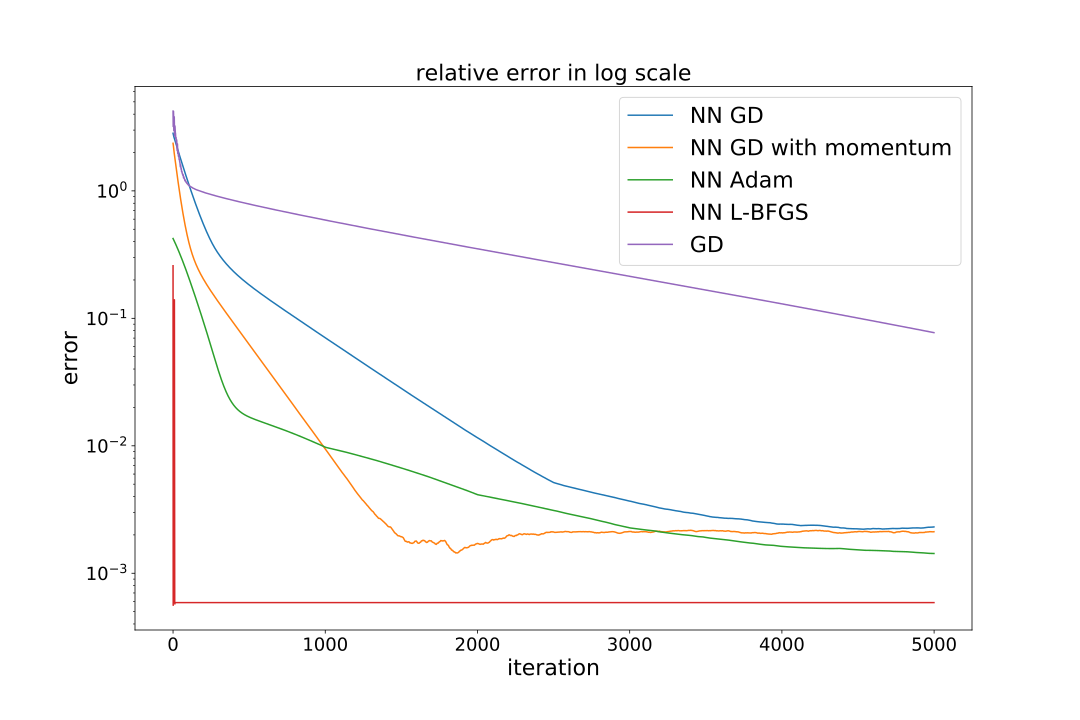
\includegraphics[width=1.1\textwidth]{figures/comparison.pdf}
\end{figure}

\medskip
\hrule\medskip
\Head{Conclusion}\\
As a result of present work, a flexible neural algorithm for solution of different calculus of variations problems has been developed. Testing has shown that it is able to achieve better precision than some naive approaches and is on par with other optimization methods for variational problems.\\\\[-1em]
Link to \href{https://github.com/suchusername/VariationalCalculus}{\underline{GitHub repository}}.


\end{textblock}

\end{document}